\section{Chapter 3 : Prediction}
The prediction problem is to find the \textbf{best possible value} for $\hat{y}(t+k|t)$ given the \textbf{measured data} up to time t $\{y(1),...,y(N)\}$
\begin{figure}[H]
 \centering
  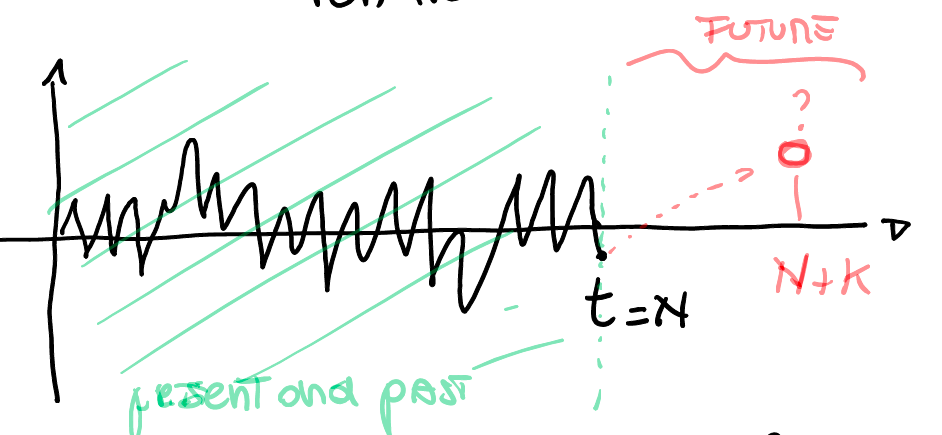
\includegraphics[width=.6\linewidth]{prediction}
\end{figure}
To obtain the \textbf{optimal} prediction :
\begin{enumerate}
\item We have to make a mathematical model for $\{y(1),..,y(N)\}$
\item Using the model compute the optimal solution
\end{enumerate}
To find the \textbf{best} mathematical model :
\begin{enumerate}
\item We select a class of models for time-series $y(t)=W(z,\theta) e(t)$ where $e(t)$ is a WN and $\theta$ a parameter vector.
\item We compute the prediction of $y(t)$ using the mathematical model : $$ \hat{y}(t+1|t;\theta) $$
\item $\hat{\theta} = argmin_{\theta}[\frac{1}{N}\sum\limits_{t=1}^{N}(y(t)-\hat{y}(t|t-1);\theta))^2]$
\item Find $y(t) = W(Z,\hat{\theta})e(t)$ which is the best model from prediction performance . Use this to compute $\hat{y}(N+K|N)$
\end{enumerate}
To create a \textbf{predictor} from an ARMA/ARMAX we need to define 2 tools:
\begin{itemize}
\item \textbf{All-pass filter}
\item \textbf{Canonical representation}
\end{itemize}

\subsection{All-Pass Filter}
An All-Pass Filter is a \textbf{first-order, linear, digital} filter with a special \textbf{constrained} structure:\\
\[
\boxed{ T(Z) = \frac{1}{a}\frac{Z+a}{Z+\frac{1}{a}} ,a \in \Re} 
\]
that depends on only one parameter and has a \textbf{pole} in $z= -\frac{1}{a}$ and zero in $z= -a$\\
Properties :\\
\begin{itemize}
\item \textbf{Magnitude}\\
$ |T(e^{jw})|^2 = |\frac{1}{a}\frac{e^{jw}+a}{e^{jw}+\frac{1}{a}}|^2 = \frac{1}{a}(\frac{e^{jw}+a}{e^{jw}+\frac{1}{a}})\cdot  \frac{1}{a}(\frac{e^{-jw}+a}{e^{-jw}+\frac{1}{a}})  = \frac{1}{a^2} \frac{1+a^2+2acosw}{1+\frac{1}{a^2}+\frac{2cosw}{a}} = 1$\\
An all-pass filter is characterized by a \textbf{frequency response} having \textbf{unitary magnitude} :
$$ \Gamma_y(w)= |T(e^{jw)}|^2 T_v(w) $$
An all-pass filter does not alter the \textbf{spectrum} of its input v(t).
This does \textbf{not} mean that $y(t) = v(t) $ but that they're \textbf{statistically equivalent} :
\[
\boxed{\Gamma_y(w) = \Gamma_v(w)}
\]
\[
\boxed{\gamma_y(w) = \gamma_v(w)}
\]
Input and output are \textbf{not} identical because although there is no change in amplitude ,an all-pass filter makes \textbf{a distortion in phase}.
\begin{figure}[H]
 \centering
  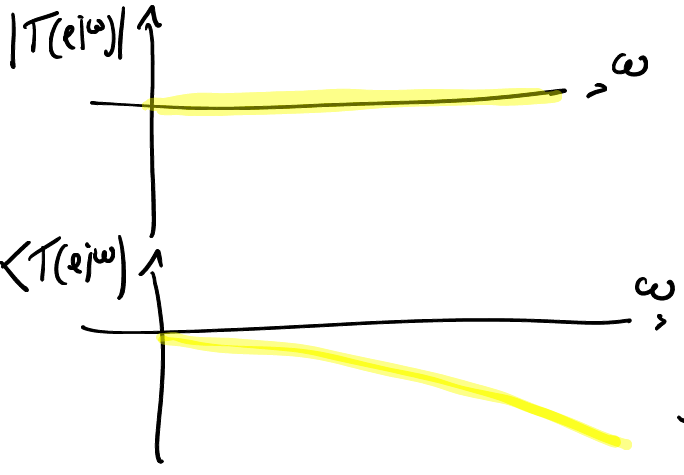
\includegraphics[width=.6\linewidth]{allpass}
\end{figure}
\begin{figure}[H]
 \centering
  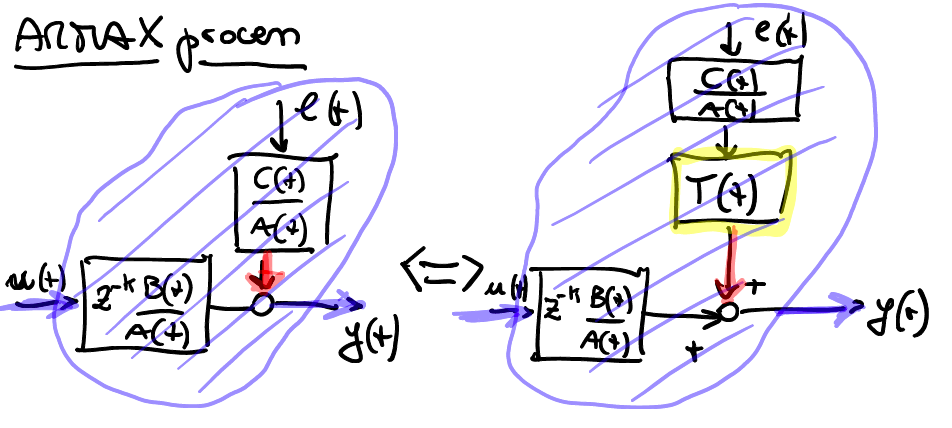
\includegraphics[width=.5\linewidth]{armaxallpass}
\end{figure}
The two representations of the ARMAX process are \textbf{equivalent}. The phase distortion added to signal e(t) is \textbf{not relevant}.
On the other hand , adding a T(Z) all-pass filter between $u(t)$ and $y(t)$ alters the behaviour of the system \textbf{critically}!!
\end{itemize}
\subsection{Canonical Representation}
An ARMA process can have $\infty$ \textbf{equivalent} representations ( there is no way to represent it in a unique way).\\
There is a special representation called \textbf{Canonical Representation}: \\
Given a SSP y(t) that can be modellded as an ARMA process: $$ y(t) = \frac{C(Z)}{A(Z)}e(t)$$ , $$ \frac{C(Z)}{A(Z)}$$ is the \textbf{canonical representation} if:
\begin{enumerate}
\item C(Z) and A(Z) have \textbf{same degree} ( relative degree is 0)
\item C(Z) and A(Z) are \textbf{coprime} ( no common factors)
\item C(Z) and A(Z) are  \textbf{monic} ( coefficient of max degree of both C(Z) and A(Z) is 1)
\item All roots of C(Z) and A(Z) are \textbf{strictly inside} the unit circle
\end{enumerate}
\begin{description}
\item[Example]\hfill\\
$ y(t) = \frac{1+3Z^{-1}}{2+Z^{-1}}e(t-2) , e(t) \sim WN(0,1)$
\begin{itemize}
\item \textbf{Type and order}\\
ARMA type process of order 1,3 = ARMA(1,3)
\item \textbf{Canonical form}\\
$$ y(t) = \frac{Z^{-2} + 3Z^{-3}}{2+Z^{-1}} e(t)$$
1. Degree of C(Z) is 2 , degree of A(Z) is 0 $\to$ X\\
2. No common factors $\to$ OK\\
3. C(Z) is monic , A(Z) is not monic $\to$ X\\
4. Zero in -3 $\to$ X \\
By collecting  and using an \textbf{All-Pass Filter}:
$$ y(t) =  \frac{Z^{-2}(1+3Z^{-1})}{2(1+\frac{1}{2}Z^{-1})} \cdot 3 \frac{1+\frac{1}{3}Z^{-1}}{1+3Z^{-1}}e(t)$$ 
\begin{figure}[H]
 \centering
  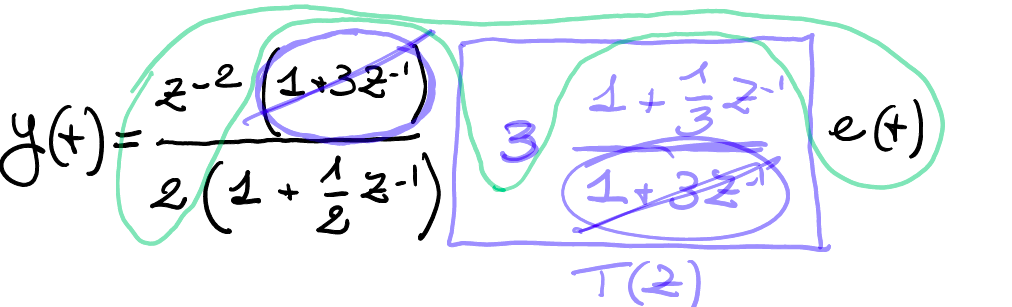
\includegraphics[width=.5\linewidth]{canonical}
\end{figure}
Defining $\theta = \frac{3}{2}e(t-2) , \theta \sim ? $\\
The variance of $\theta = E[\theta(t)^2]= E[(\frac{3}{2}e(t-2))^2] = \frac{9}{4}\cdot 1$\\
$\theta \sim WN(0,\frac{9}{4}) ? \to$ $ \Gamma_\theta(w)= |\frac{3}{2}e^{-2jw}|^2 \cdot 1 = \frac{9}{4} $ which is constant value so $\theta \sim WN(0,\frac{9}{4})$
Finally we obtain : 
\[
\boxed{y(t) =\frac{1+\frac{1}{3}Z^{-1}}{1+\frac{1}{2}Z^{-1}}\theta(t) , \theta \sim WN(0,\frac{9}{4})}
\]
Which is an \textbf{ARMA(1,1)} $\to$ the \textbf{canonical representation} is the representation with \textbf{minimum order!}
\end{itemize}

\item[Remark]\hfill\\
Does the canonical representation \textbf{always} exist?\\
Not always :  the problem lies in the $4^{th}$ condition . It is possible that the system has poles or zeros \textbf{on} the unitary circle.
\begin{figure}[H]
 \centering
  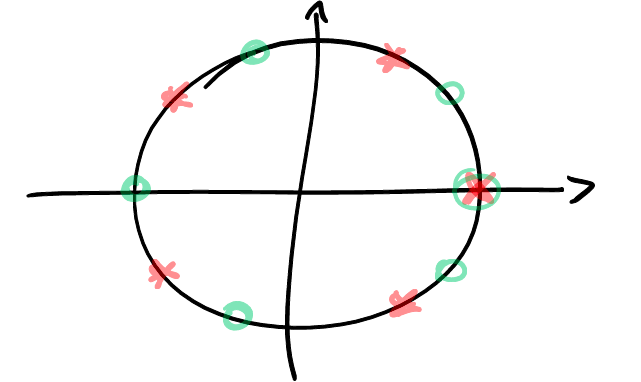
\includegraphics[width=.5\linewidth]{remark_simple}
\end{figure}
If $C(Z)$ has \textbf{zeros on the u.c} $\to$ prediction from data is \textbf{not asymptotically stable}\\
If $A(Z)$ has \textbf{roots in +1} $\to$ \textbf{ARIMA models}:
\[
\boxed{y(t) = \frac{C(Z)}{(Z-1)^dA(Z)}e(t) \to ARIMA(m,d,n)}
\]
[Autoregressive Integrated Moving average ]\\
A special case of ARIMA $\to$ \textbf{ARIMA(0,1,0)}:
\[
\boxed{y(t) = \frac{1}{1-Z^{-1}}e(t)}
\]
\[
\boxed{y(t) =y(t-1) +e(t) , e(t) \sim WN(0,\lambda^2)}
\]
Process y(t) is a \textbf{Random Walk} that uses as TF $\frac{1}{1-Z^{-1}}$ which is an \textbf{integrator in discrete time}
\end{description}
ARIMA processes have an \textbf{asymptotically stable} predictor that can be used to model \textbf{not strictly stationary processes!!}

\subsection{Predictor}
The predictor at time t+k , given the data up to time t is:
$$ \hat{y}(t+k|t) $$
The \textbf{prediction error} is: 
$$  \epsilon(t+k) = y(t+k)- \hat{y}(t + k|t)$$
So the \textbf{real value } is predictor + error:
$$ y(t+k|t) = \hat{y}(t+k|t) + \epsilon(t+k)$$
$$ y(t) = \hat{y}(t|t-k) + \epsilon(t) $$
The formulas as equivalent because as per hypothesis $y(t)$ is \textbf{stationary}.
\subsubsection{Optimality}
The predictor $ \hat{y}(t+k|t) $ is \textbf{optimal} if:
\begin{enumerate}
\item $ E[\hat{y}(t+k|t) \cdot \epsilon(t+k)]=0 $ , predictor and error must be \textbf{incorrelated}
\item $ E[y(t) \cdot \epsilon(t+k)] = E[y(t-1) \cdot \epsilon(t+k)]... = 0$
\end{enumerate}
\begin{figure}[H]
 \centering
  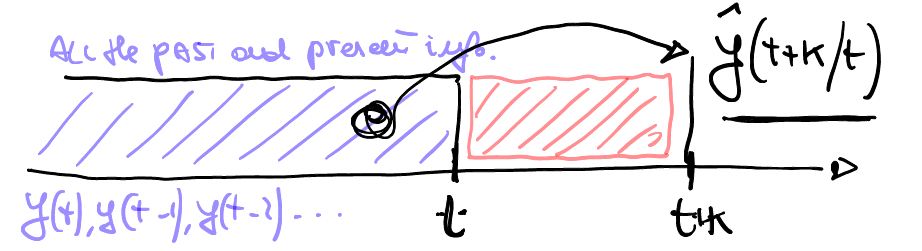
\includegraphics[width=.5\linewidth]{predictoropt}
\end{figure}
The red part shows the \textbf{unpredictable} part of y(t+k) , which is the error $\epsilon(t+k)$. If error and predictor were \textbf{correlated} than some useful unused information about $\hat{y}(t+k|t)$ would be in $\epsilon(t+k)$ which means that the predictor is not optimal.\\
The same goes for $y(t) , y(t-1)...$ of point 2): the error cannot contain information about the past/present information.\\

\subsubsection{1-step ahead prediction of MA(n)}
$$ y(t) = e(t) + c_1e(t-1)+...+c_ne(t-n) , e(t) \sim WN(0,\lambda^2)$$
We assume the the MA(n) is represented in the \textbf{canonical representation} : we must make assumptions about the $4^{th}$ property.\\
Given :\\
- \textbf{Present time} : t-1 $\to c_1e(t-1)+...+c_ne(t-n)$\\
- \textbf{Future} : t $\to e(t)$\\
\begin{description}
\item[Predictor from noise]\hfill\\
The \textbf{optimal predictor} from \textbf{noise} is :
\[
\boxed{\hat{y}(t|t-1)=c_1e(t-1)+...+c_ne(t-n)}
\]
with error 
\[
\boxed{\epsilon(t) = y(t) - \hat{y}(t|t-1) = e(t)}
\]
Optimality :
\begin{itemize}
\item $E[\hat{y}(t|t-1)\epsilon(t)]= E[(c_1e(t-1)+...+c_ne(t-n))(e(t))]=0 $
\item $E[y(t-1)\epsilon(t)]=E[(e(t-1)+c_1e(t-2)+...+c_ne(t-n-1))(e(t))]=...=0$ 
\end{itemize}
Verified because of incorrelation of white noise.\\
Since WN is \textbf{unknown} and cannot be measured , a better predictor has to be chosen from \textbf{measurable data}.

\item[Predictor from data]\hfill\\
TF:
$$ y(t) = (1+c_1Z^{-1}+...+c_nZ^{-n})e(t)$$
Inverse TF (\textbf{Whitening Filter}):
$$ e(t) = \frac{1}{1+c_1Z^{-1}+...+c_nZ^{-n}}y(t)$$
$$ \hat{y}(t|t-1) = (1+c_1Z^{-1}+...+c_nZ^{-n})e(t) \to \hat{y}(t|t-1) = \frac{c_1Z^{-1}+...+c_nZ^{-n}}{1+c_1Z^{-1}+...+c_nZ^{-n}}y(t) $$
Collecting $Z^{-1}$ :
\[
\boxed{\hat{y}(t|t-1) = \frac{c_1+...+c_nZ^{-n+1}}{1+c_1Z^{-1}+...+c_nZ^{-n}}y(t-1)}
\]
\begin{figure}[H]
 \centering
  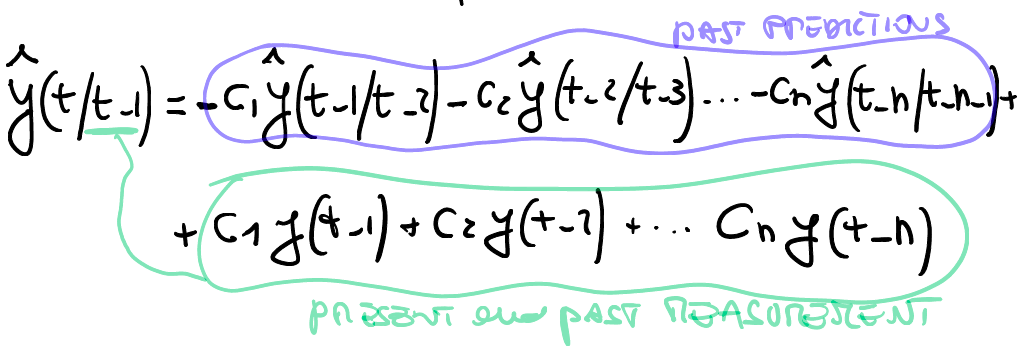
\includegraphics[width=.5\linewidth]{mapredictor}
\end{figure}
As seen in time-domain representation the prediction makes use of \textbf{present and past} data as well as \textbf{past predictions}.
\end{description}

\subsubsection{K-steps ahead predictor of MA(n)}
$$ y(t) = e(t)+c_1e(t-1)+...+c_{k-1}e(t-k+1)+c_ke(t-k)+...+c_ne(t-n)$$
Given:\\
-\textbf{Present time}: k $\to c_ke(t-k)+...+c_ne(t-n)$\\
-\textbf{Future} : t $\to e(t)+...+c_{k-1}e(t-k+1)$\\
\begin{description}
\item[Predictor from noise]\hfill\\
\[
\boxed{\hat{y}(t|t-k)=c_ke(t-k)+...+c_ne(t-n)}
\]
with error:
\[
\boxed{\epsilon(t)=e(t)+...+c_{k-1}e(t-k+1)}
\]
\item[Predictor from data]\hfill\\
\[
\boxed{\hat{y}(t|t-k)=\frac{c_k+c_{k+1}Z^{-1}+...+c_nZ^{-n+k}}{1+c_1Z^{-1}+...+c_nZ^{-n}}y(t-k)}
\]
\end{description}

\subsubsection{K-steps ahead predictor of general ARMA(m,n)}
$$ y(t) = \frac{C(Z)}{A(Z)}e(t) , e(t) \sim WN(0,\lambda^2)$$
(Under the hypothesis of \textbf{canonical representation})\\
The AR(m) part presents a recursion : need to introduce k-steps \textbf{polynomial division} between C(Z) and A(Z) obtaining :\\
- \textbf{E(Z)} $\to$ result (quotient)\\
- \textbf{R(Z)} $\to$ residual (remainder) \\
\begin{figure}[H]
 \centering
  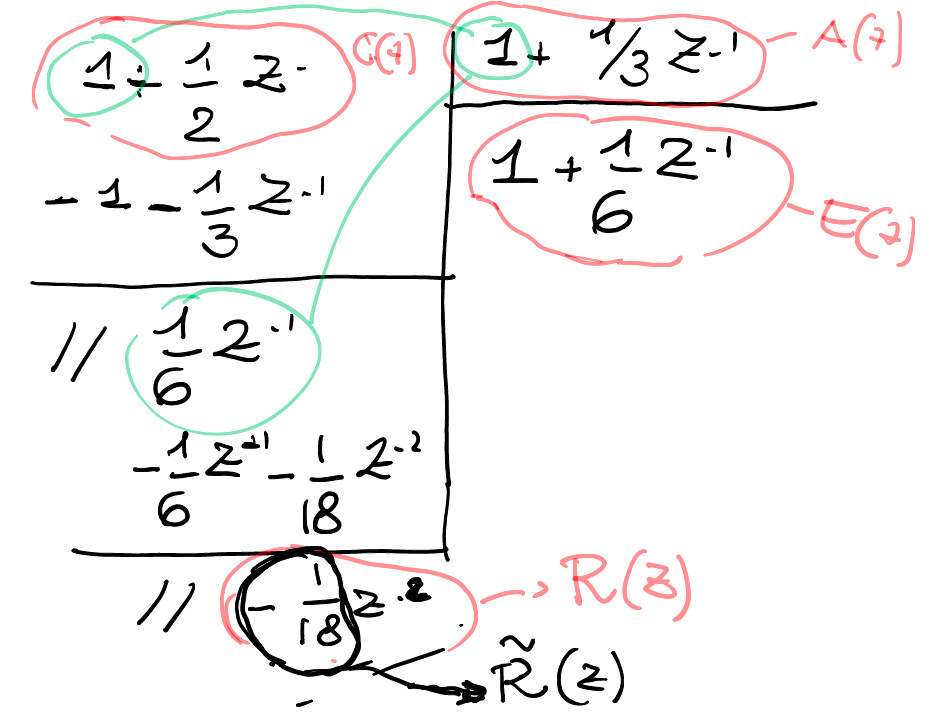
\includegraphics[width=.7\linewidth]{poldivision}
\end{figure}
$$C(Z)=E(Z)A(Z) + R(Z)$$
\[
\boxed{ \frac{C(Z)}{A(Z)}=E(Z) + \frac{R(Z)}{A(Z)}}
\]
Noting that in k-steps division R(Z) can be rewritten by collecting $Z^{-k}$: 
$$ R(Z) = Z^{-k}\tilde{R}(Z)$$
\[
\boxed{ \frac{C(Z)}{A(Z)}=E(Z) + \frac{Z^{-k}\tilde{R}(Z))}{A(Z)}}
\]
The new transfer function is: 
$$ y(t) = [E(Z) + \frac{Z^{-k}\tilde{R}(Z))}{A(Z)}] e(t) $$
$$ y(t) = E(Z)e(t) + \frac{\tilde{R}(Z))}{A(Z)} e(t-k) $$
Where $ E(Z)e(t) $ is the \textbf{unpredictable part} as it depends on 
$ e(t) ,...,e(t-k+1)$

\begin{description}
\item[Predictor from noise]\hfill\\
\[
\boxed{\hat{y}(t|t-k) = \frac{\tilde{R}(Z)}{A(Z)}e(t-k)}
\]
with error:
\[
\boxed{\epsilon(t) = E(Z)e(t)}
\]
\item[Predictor from data]\hfill\\
$$ y(t) =\frac{C(Z)}{A(Z)}e(t) \xrightarrow[\text{Whitening}]{}e(t) = \frac{A(Z)}{C(Z)}y(t)$$
$$ \hat{y}(t|t+k) = \frac{\tilde{R}(Z)Z^{-k}}{A(Z)} \cdot \frac{A(Z)}{C(Z)}y(t)$$
\[
\boxed{\hat{y}(t|t-k) = \frac{\tilde{R}(Z)}{C(Z)}y(t-k)}
\]
\item[Remark 1]\hfill\\
Both the predictor from noise and data work under the assumption of SSP . The stationary property is satisfied if both A(Z) and C(Z) have all roots (poles) strictly inside the unitary circle. But this is satisfied by the $4^{th}$ condition of the canonical representation hypothesis.
\item[Remark 2]\hfill\\
$\epsilon(t) = y(t)- \hat{y}(t|t-k)=E(Z)e(t)$ where $E(Z)$ is a SSP of type \textbf{MA(k-1)}
\item[Remark 3]\hfill\\
In the case of \textbf{K=1} the polynomial division result in :\\
-\textbf{E(Z)} = 1 as both C(Z),A(Z) are monic and have same degree\\
-\textbf{R(Z)} = C(Z)-A(Z)\\
which results in 
\[
\boxed{\hat{y}(t|t-k)=\frac{C(Z)-A(Z)}{A(Z)}e(t)}
\]
\[
\boxed{\hat{y}(t|t-k)=\frac{C(Z)-A(Z)}{C(Z)}y(t)}
\]
\[
\boxed{\epsilon(t)=e(t)}
\]
Instead of having term R(Z) , the formula is now C(Z)-A(Z). As $R(Z)= \tilde{R}(Z)Z^{-1}$ there is a hidden $Z^{-1}$ in C(Z)-A(Z).
\end{description}

\subsubsection{K-steps ahead prediction of ARMAX(m,n,k+p)}
$$ y(t) = \frac{B(Z)}{A(Z)}u(t-k) + \frac{C(Z)}{A(Z)}e(t) ,e(t) \sim WN(0,\lambda^2)$$
Where:
$$ A(Z)=1+a_1Z^{-1}+...+a_mZ^{-m}$$
$$ B(Z)=b_0 + b_1Z^{-1}+...+b_pZ^{-p}$$
$$ C(Z)=1+c_1Z^{-1}+...+c_nZ^{-n}$$
In the hypothesis that $\frac{C(Z)}{A(Z)}$ is in \textbf{canonical representation} and keeping in mind that for $\frac{B(Z)}{A(Z)}u(t-k)$ no \textbf{spectral equivalence} modifications can be made.\\
In an ARMAX(m,n,k+p) process the most interesting prediction that can be made is the \textbf{delay} between u(t) and y(t) $\to$ \textbf{k} so we'll deal only with k-steps predictions.
\begin{description}
\item[Predictor from noise]\hfill\\
Separate predictable from unpredictable part in $\frac{C(Z)}{A(Z)}e(t)$\\
K-steps division $\frac{C(Z)}{A(Z)} \to E(Z)+\frac{R(Z)}{A(Z)}$
$$ y(t) = \frac{B(Z)}{A(Z)}u(t-k) + E(Z)e(t) + \frac{\tilde{R}(Z)}{A(Z)}e(t-k)$$
where 
$$\frac{B(Z)}{A(Z)}u(t-k) \to \text{depends on } u(t-k),...,u(t-k-p) \to \text{predictable} $$ 
$$ E(Z)e(t) \to \text{depends on } e(t) , e(t-1),...,e(t-k+1) \to \text{unpredictable} $$ 
$$ \frac{\tilde{R}(Z)}{A(Z)}e(t-k) \to \text{depends on } e(t-k),...,e(t-k-p) \to \text{predictable}$$   
so
\[
\boxed{\hat{y}(t|t-k)=\frac{B(Z)}{A(Z)}u(t-k)+\frac{R(Z)}{A(Z)}e(t)}
\]
\[
\boxed{\epsilon(t) = y(t) - \hat{y}(t|t-k) = E(t)e(t)}
\]
Which is optimal if\begin{itemize}
\item $\epsilon(t) \perp \hat{y}(t|t-k)$
\item $\epsilon(t) \perp y(t-k),y(t-k-1)... $
\end{itemize}

\item[Predictor from data]\hfill\\
$$ e(t) = \frac{A(Z)}{C(Z)}y(t) - \frac{B(Z)}{A(Z)}u(t-k)$$
$$ \hat{y}(t|t-k) = \frac{B(Z)}{A(Z)}u(t-k)+ \frac{R(Z)}{A(Z)} [\frac{A(Z)}{C(Z)}y(t)- \frac{B(Z)}{A(Z)}u(t-k)]$$
$$ \hat{y}(t|t-k) = \frac{R(Z)}{C(Z)}y(t) + [\frac{B(Z)}{A(Z)}-\frac{R(Z)B(Z)}{A(Z)C(Z)}]u(t-k)$$
$$ \hat{y}(t|t-k) = \frac{B(Z)}{C(Z)}y(t) + [\frac{B(Z)(C(Z)-R(Z))}{A(Z)C(Z)}]u(t-k)  $$
Knowing that $C(Z)= A(Z)E(Z)+R(Z) \to C(Z)-R(Z)= A(Z)E(Z)$
\[
\boxed{\hat{y}(t|t-k)=\frac{B(Z)E(Z)}{C(Z)}u(t-k) + \frac{\tilde{R}(Z)}{C(Z)}y(t-k)}
\]
\[
\boxed{\epsilon=E(Z)e(t)}
\]
Note that $\frac{\tilde{R}(Z)}{C(Z)}y(t-k) $ is the exact ARMA predictor.\\
The prediction error is the same as in the \textbf{ARMA} process: the \textbf{exogenous} part does not add any \textbf{additional uncertainty}.

\item[Remark : Special case k=1]\hfill\\
$$ y(t) = \frac{B(Z)}{A(Z)}u(t-1)+\frac{C(Z)}{A(Z)}e(t)$$
$E(Z) =1 $ and $ R(Z)= C(Z)-A(Z)$
$$ \hat{y}(t|t-1)= \frac{B(Z)}{C(Z)}u(t-1) + \frac{C(Z)-A(Z)}{C(Z)}y(t)$$

\end{description}

\subsection{Examples \& Exercises}

\subsubsection{Example 1}
Given a process $$ y(t)= \frac{Z+3}{2Z+1} e(t-1) , e(t) \sim WN(0,1)$$
Since the pole of the TF is $z=-\frac{1}{2}$ inside the unitary circle ,  W(Z) is asymptotically stable $\to$ y(t) is \textbf{stationary}.\\
\begin{enumerate}

\item \textbf{Compute $\gamma_y(0)$}\\
NB.: To calculate the variance it is not important fort the system to be in canonical representation\\
$y(t) = \frac{C(Z)}{A(Z)}e(t-1) $ is \textbf{not canonical} since it has \\
- Z = -3 not inside unitary circle\\
- 2Z in the A(Z) term\\
- $Z^{-1}e(t)$\\
Using an \textbf{All-Pass Filter}: 
$$ y(t) = \frac{Z+3}{2(Z+\frac{1}{2})} Z^{-1} \cdot 3 \frac{Z+\frac{1}{3}}{Z+3}e(t)$$
$$ \eta = \frac{3}{2}Z^{-1}e(t) \sim WN(0,\frac{9}{4}$$
$$ y(t) = \frac{Z+\frac{1}{3}}{Z+\frac{1}{2}}\eta(t)$$
Passing in time domain : $$ y(t)= -\frac{1}{2}y(t-1)+\eta(t) +\frac{1}{3}\eta(t-1)$$
-$m_y = E[y(t)]= -\frac{1}{2}E[y(t-1)]+\frac{4}{3}m_e \to 0$\\
-$\gamma_y(0) = E[y(t)^2] = E[(-\frac{1}{2}y(t-1) + \eta(t) + \frac{1}{3}\eta(t-1))^2]$\\
  $\gamma_y(0) = \frac{1}{4}\gamma_y(0) + \frac{9}{4} + \frac{1}{9}\frac{9}{4} - \frac{1}{3}E[y(t-1)\eta(t-1)]$\\
  $\frac{3}{4}\gamma_y(0) =\frac{10}{4} - \frac{1}{3}E[(-\frac{1}{2}y(t-2)+\eta(t-1)+\frac{1}{3}\eta(t-2))\eta(t-1)] $\\
  $\frac{3}{4}\gamma_y(0) = \frac{10}{4} -\frac{1}{3}E[\eta(t-1)^2] \to \frac{3}{4}\gamma_y(0) = \frac{10}{4} -\frac{1}{3}\frac{9}{4}$
 \[
 \boxed{\gamma_y(0)=\frac{7}{3}}
 \]

\item \textbf{Prediction for k=1}\\
Using the canonical negative power representation $$ y(t) = \frac{1+\frac{1}{3}Z^{-1}}{1+\frac{1}{2}Z^{-1}}\eta(t)$$
Applying the k=1 prediction formula $ \hat{y}(t|t-1) = \frac{C(Z)-A(Z)}{C(Z)}y(t)$ :
$$ \hat{y}(t|t-1) = \frac{1+\frac{1}{3}Z^{-1}-1-\frac{1}{2}Z^{-1}}{1+\frac{1}{3}Z^{-1}}y(t)$$
$$ \hat{y}(t|t-1) = \frac{-\frac{1}{6}}{1+\frac{1}{3}Z^{-1}}y(t-1)$$
In time domain :
\[
\boxed{\hat{y}(t|t-1) = -\frac{1}{3}\hat{y}(t-1|t-2)-\frac{1}{6}y(t-1)}
\]
\[
\boxed{\epsilon(t) = y(t) - \hat{y}(t|t-1) = E(Z)\eta(t) = \eta(t)}
\]
\[
\boxed{var[ y(t) - \hat{y}(t|t-1)]= var[\eta(t)] = \frac{9}{4}}
\]
\newpage
\item \textbf{Prediction for k=2}
\begin{figure}[H]
 \centering
  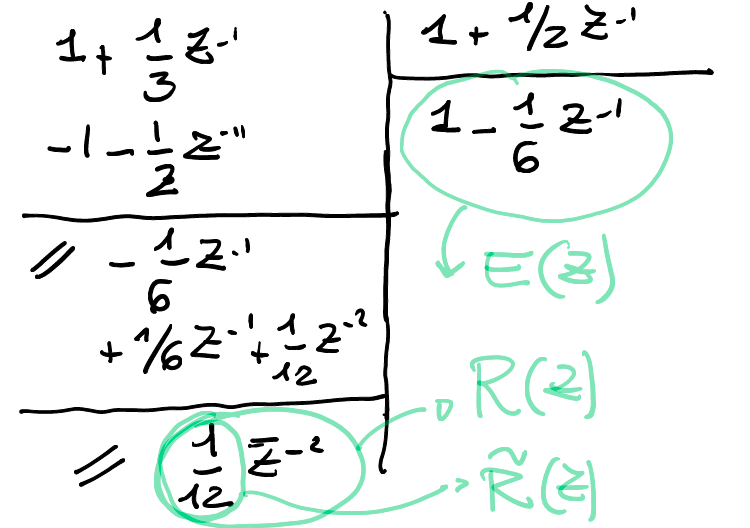
\includegraphics[width=.5\linewidth]{ex_division}
\end{figure}
$$ \hat{y}(t|t-2) = \frac{R(Z)}{C(Z)}y(t) = \frac{\tilde{R}(Z)}{C(Z)}y(t-2)$$
$$ \hat{y}(t|t-2) = \frac{\frac{1}{12}}{1+\frac{1}{3}Z^{-1}}y(t-2)$$
\[
\boxed{\hat{y}(t|t-2) = -\frac{1}{3}\hat{y}(t-1|t-3) +\frac{1}{12}y(t-2)}
\]
\[
\boxed{\epsilon(t) = y(t) - \hat{y}(t|t-2) = E(Z)\eta(t) = (1-\frac{1}{6}Z^{-1})\eta(t)}
\]
\[
\boxed{var[ y(t) - \hat{y}(t|t-2)]= var[(1-\frac{1}{6}Z^{-1})\eta(t)] = \frac{37}{16}}
\]
\newpage
\item \textbf{Properties of $var[\epsilon(t)]$ as function of $k$}
\begin{figure}[H]
 \centering
  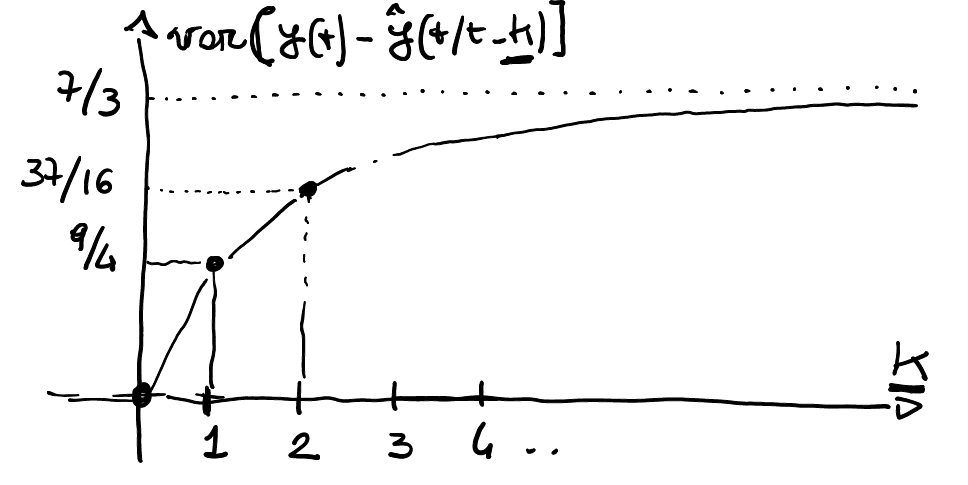
\includegraphics[width=.5\linewidth]{ex_vark}
\end{figure}
- $k=0 \to var[y(t) -\hat{y}(t|t-k)] = 0$\\
- $k=1 \to var[y(t) -\hat{y}(t|t-k)] = \lambda^2$\\
- $k \to \infty \to var[y(t) -\hat{y}(t|t-k)] = \gamma_y(0)$ because when $k \to \infty$ the prediction goes to zero!\\
- $ var[y(t) -\hat{y}(t|t-k)] $ is a \textbf{monotonic (not strictly) increasing} function

\item \textbf{Prediction goodness}\\
The \textbf{Error to signal ratio} is a useful prediction measure:
$$ ESR(k) = \frac{var[y(t) - \hat{y}(t|t-k)]}{var[y(t)]}$$
For k=1 $$ESR(1) = \frac{\frac{9}{4}}{\frac{7}{3}} = 0.97$$
Which is a very bad prediction. The most trivial prediction that can be done is 
$$ \hat{y}(t|t-k) = m_y$$  (predicting the mean) which has \textbf{ESR(k)=1}.\\
For k=1 we only have a 3\% better prediction than the trivial one.\\
The predictor for k=1 is \textbf{optimal} which means that \textbf{no better } prediction can be made : the bad prediction is an intrinsic property of the process y(t).\\
 
\begin{figure}[H]
\begin{minipage}{.5\textwidth}
 \centering
  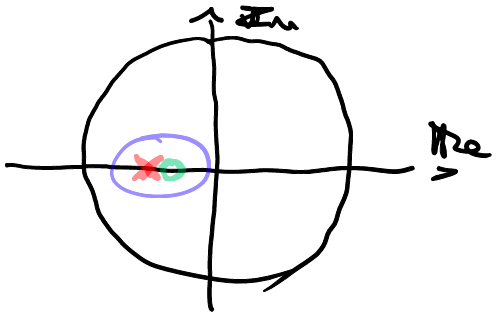
\includegraphics[width=.6\linewidth]{ex_poles}
\end{minipage}%
	\begin{minipage}{.5\textwidth}
  \centering
  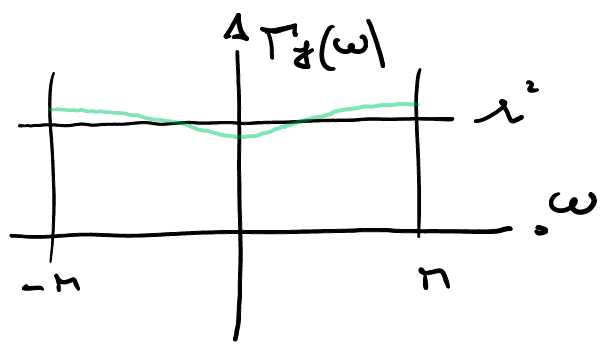
\includegraphics[width=.9\linewidth]{ex_spectrum}
\end{minipage}%
\end{figure}
By analysing the poles and zeros, it is easy to see that they're so close together that they almost cancel each other out.\\
The \textbf{spectrum} $\Gamma_y(w)$  in green is very close to that of the \textbf{white noise}: this is the reason y(t) is hard to predict 
\end{enumerate}


\subsubsection{Example 2 - Practical}
We have measured 5 data points of a signal: \\ $ y(1)=1, y(2) =\frac{1}{2}, y(3) =-\frac{1}{2}, y(4)=0, y(5)= -\frac{1}{2}$\\
With t=5 represent the present time  , make a prediction of $ \hat{y}(6|5) $.
To solve the problem we must make a mathematical modelling assumption. Since we're still not able to do this we need some interpretations models for this signal\\
Model A $$ y(t) = \frac{1}{2}y(t-1)+\frac{1}{4}y(t-2)+e(t) , e(t) \sim WN(0,\lambda^2)$$
Model B $$ y(t) = e(t) +\frac{1}{2}e(t-1),e(t) \sim WN(0,\lambda^2)$$
To determine which model is better we compute the \textbf{optimal} model assuming the chosen model is right.
\begin{itemize}
\item \textbf{Assuming Model A right}\hfill\\
$$ y(t) = \frac{1}{1-\frac{1}{2}Z^{-1}-\frac{1}{4}Z^{-2}} e(t)$$ is an AR(2) process in canonical representation (check it always!).\\
Since we're dealing with a k=1 prediction : 
$$ \hat{y}(t|t-1) = \frac{C(Z)-A(Z)}{C(Z)}y(t)$$
$$ \hat{y}(t|t-1) = \frac{1-1+\frac{1}{2}Z^{-1}+\frac{1}{4}Z^{-2}}{1}y(t)$$
$$ \hat{y}(t|t-1) = \frac{1}{2}y(t-1) + \frac{1}{4}y(t-2)$$
Substituting the data points :
$$ \hat{y}(6|5) = \frac{1}{2}y(5) + \frac{1}{4}y(4) = -\frac{1}{4}$$
\item \textbf{Assuming Model B right}\hfill\\
$$ y(t) = (1+\frac{1}{2}Z^{-1})e(t) $$ is an MA(1) process in canonical representation.\\
Since we're dealing with a k=1 prediction : 
$$ \hat{y}(t|t-1) = \frac{C(Z)-A(Z)}{C(Z)}y(t)$$
$$ \hat{y}(t|t-1) = \frac{1+\frac{1}{2}Z^{-1}-1}{1+\frac{1}{2}Z^{-1}}y(t)$$
$$ \hat{y}(t|t-1) = -\frac{1}{2}\hat{y}(t-1|t-2) +\frac{1}{2}y(t-1)$$
Substituting the data points :
$$ \hat{y}(6|5) = -\frac{1}{2}\hat{y}(5|4) + \frac{1}{2}y(5) = -\frac{1}{2}\hat{y}(5|4) -\frac{1}{4}$$
To compute $-\frac{1}{2}\hat{y}(5|4)$ we need to go back to the \textbf{initial condition } to compute all terms up to time =5:\\
-$ \hat{y}(2|1) = -\frac{1}{2}\hat{y}(1|0) + \frac{1}{2}y(1)$ by making the assumption that $-\frac{1}{2}\hat{y}(1|0) = m_y \to \frac{1}{2}$\\
-$ \hat{y}(3|2) = -\frac{1}{2}\hat{y}(2|1) + \frac{1}{2}y(2) = 0$\\
-$ \hat{y}(4|3) = -\frac{1}{2}\hat{y}(3|2) + \frac{1}{2}y(3) = -\frac{1}{4}$\\
-$ \hat{y}(5|4) = -\frac{1}{2}\hat{y}(4|3) + \frac{1}{2}y(4) = \frac{1}{8}$\\
-$ \hat{y}(6|5) = -\frac{1}{2}\hat{y}(5|4) + \frac{1}{2}y(5) = -\frac{5}{16}$\\
Our final prediction for model B is $\hat{y}(6|5) = -\frac{5}{16}$ which depends on the initial condition made assuming that $-\frac{1}{2}\hat{y}(1|0) = m_y $. It the choice of the initial condition important?
\textbf{If the system is asymptotically stable, and N is big the initial condition is not important as it will vanish.}

\subsubsection{Example 3 - ARMAX \& ARX}
$$ y(t) = (Z+6Z^{-1})u(t-2) + \frac{2}{3+\frac{3}{2}Z{-1}}\eta(t-1) , \eta \sim WN(0,1)$$
Find predictor from data and the corresponding error with its variance.\\
u(t-2) $\to$ k=2\\
Canonical form for ARMA part\\
$$ \frac{2}{3(1+\frac{1}{2}Z^{-1})}Z^{-1}\eta(t)$$
So $$ e(t) = \frac{2}{3} \eta(t-1) , e(t) \sim WN(0,\frac{4}{9}$$
$$ \frac{1}{1+\frac{1}{2}Z^{-1}}e(t)$$
Substituting in the original process:
$$ y(t) = (Z+6Z^{-1})u(t-2) +  \frac{1}{1+\frac{1}{2}Z^{-1}}e(t), e(t) \sim WN(0,\frac{4}{9})$$
Is the term $(Z+6Z^{-1})u(t-2)$ also in canonical representation? Wrong question, there is nothing we can do about it!\\
We need the form : $$ y(t) = \frac{B(Z)}{A(Z)}u(t-k) + \frac{C(Z)}{A(Z)}e(t)$$
So rewriting :
$$ y(t) =\frac{(2+6Z{-1})(1+\frac{1}{2}Z^{-1})}{(1+\frac{1}{2}Z^{-1})}u(t-2)+ \frac{1}{1+\frac{1}{2}}e(t)$$
Using a k-steps long division $\frac{C(Z)}{A(Z)}$:
\begin{figure}[H]
 \centering
  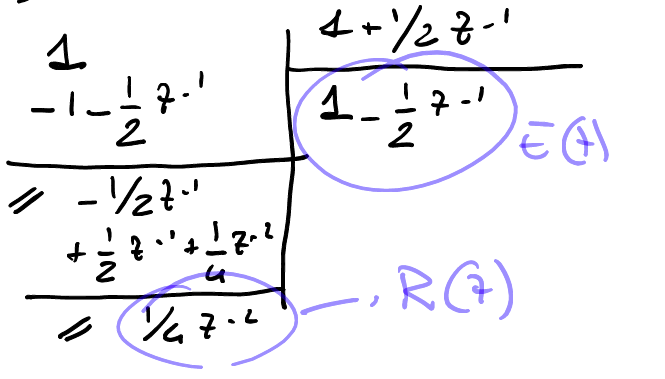
\includegraphics[width=.5\linewidth]{ex_division2}
\end{figure}
\end{itemize}
$$ \hat{y}(t|t-2) = \frac{(2+6Z^{-1})(1+\frac{1}{2}Z^{-1})(1-\frac{1}{2}Z{-1})}{1}u(t-2)+ \frac{\frac{1}{4}Z^{-2}}{1} y(t)$$

\[
\boxed{\hat{y}(t|t-2) = 2u(t-2)+6u(t-3)-\frac{1}{2}u(t-4)-\frac{3}{2}u(t-5)+\frac{1}{4}y(t-2)}
\]
\textbf{No old prediction} is used $\to$ process is \textbf{ARMAX(1,0,2+2)} $\to$ \textbf{ARX(1,4)} model.
\[
\boxed{\epsilon=E(Z)e(t)=(1-\frac{1}{2})Z^{-1}e(t)}
\]
The variance of $\epsilon$ :
$$ var[\epsilon(t)]= (1+\frac{1}{4})\cdot \frac{4}{9} = \frac{5}{4}\frac{4}{9}= \frac{5}{9}$$


\subsubsection{Example ARMA with non-zero mean}
$$ y(t) =e(t) + 4e(t-1) , e \sim WN(1,1)$$
Compute $\hat{y}(t|t-1)$ and $\hat{y}(t|t-2)$ from data.\\
Canonical form representation\\
$$y(t) =(1+4Z^{-1})e(t) \to y(t)= (1+4Z^{-1})[4\cdot \frac{1+\frac{1}{4}Z^{-1}}{1+4Z^{-1}}]e(t)$$
Getting the new $\eta(t)$:
$$ \eta(t) = 4e(t)$$
$$m_{\eta}=E[\eta(t)]=E[4e(t)] = 4$$
$$var[\eta]= E[(\eta(t)-4)^2]= E[(4e(t)-4)^2]= 16E[(e(t)-1)^2] =16$$
Canonical form :
\[
\boxed{y(t) =(1+\frac{1}{4}Z^{-1})\eta(t)}
\]
\[
\boxed{\eta(t) \sim WN(4,16)}
\]
\begin{description}
\item[Method 1]\hfill\\
\textbf{De-biasing technique}:
$$ \tilde{y}(t) = y(t) - m_y$$
$$ \tilde{\eta}(t) = \eta(t) - m_{\eta}$$
Mean of y:
$$ E[y(t)]=E[(\eta(t)+\frac{1}{4}\eta(t-1))] \to m_y= \frac{5}{4}m_{\eta}=5$$
So:
$$ \tilde{y}(t) = y(t) - 5$$
$$ \tilde{\eta}(t) = \eta(t) - 4 \to \tilde{\eta} \sim WN(0,16)$$
Obtaining:
$$ \tilde{y}+5= (\tilde{\eta}(t)+4)+\frac{1}{4}(\tilde{\eta}(t-1)+4)$$
\[
\boxed{\tilde{y}= \tilde{\eta}(t)+\frac{1}{4}\tilde{\eta}(t-1)}
\]
Now we can compute the predictions for $\tilde{y}$ for k=1:
 $$ \hat{\tilde{y}}(t|t-1)= \frac{(1+\frac{1}{4}Z^{-1})-1}{(1+\frac{1}{4}Z{-1})} \tilde{y}(t)$$
\[
\boxed{\hat{\tilde{y}}(t|t-1)= \frac{\frac{1}{4}}{(1+\frac{1}{4}Z{-1})} \tilde{y}(t-1)}
\]
\[
\boxed{\epsilon(t) = \tilde{\eta}(t) = 16}
\]
Now we can compute the prediction for $\tilde{y}$ for k=2:
\begin{figure}[H]
 \centering
  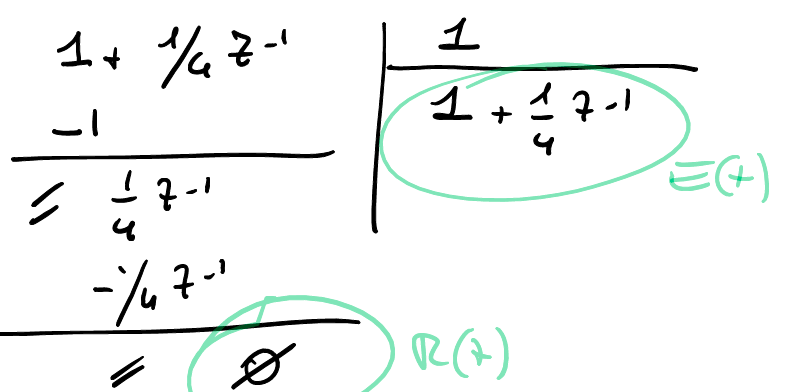
\includegraphics[width=.5\linewidth]{ex_division3}
\end{figure}
Which means that 
\[
\boxed{\hat{\tilde{y}}(t|t-2) = 0}
\]
Because MA(1) process has a \textbf{finite memory} of 1-step only!
So $\tilde{\epsilon}(t) = \tilde{y}(t) - \hat{\tilde{y}}(t|t-2) = \tilde{y})(t)$ so the $var[\tilde{\epsilon}(t)]=var[\tilde{y}(t)] = (1+\frac{1}{16}) \cdot 16= 17$
\begin{figure}[H]
 \centering
  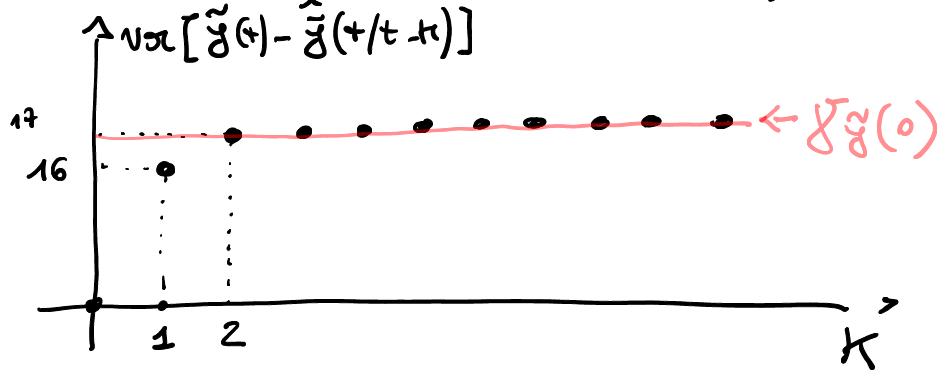
\includegraphics[width=.5\linewidth]{ex_varplot}
\end{figure}
We need to go back to the original process because $\hat{y}(t|t-1) \neq \hat{\tilde{y}}(t|t-1)$ : 
- for \textbf{k=1}\\
$$ \hat{y}(t|t-1)-5 = \frac{\frac{1}{4}}{1+\frac{1}{4}Z^{-1}}(y(t-1)-5)$$
$$ \hat{y}(t|t-1)= \frac{\frac{1}{4}}{1+\frac{1}{4}Z^{-1}}y(t-1)+5 - 5\frac{\frac{1}{4}}{1+\frac{1}{4}Z^{-1}}$$
The term  $5\frac{\frac{1}{4}}{1+\frac{1}{4}Z^{-1}}$ can be resolved by applying the \textbf{frequency response theorem } by taking in account that $5$ is a sinusoid with frequency $w=0$ : 

$$ \frac{\frac{1}{4}}{1+\frac{1}{4}e^{0j}} \cdot 5 = 1$$ 
so :
\[
\boxed{\hat{y}(t|t-1)= \frac{\frac{1}{4}}{1+\frac{1}{4}Z^{-1}}y(t-1)+4}
\]
- for \textbf{k=2}\\
$$ \hat{\tilde{y}}(t|t-2) = 0 \to \hat{y}(t|t-2) -5= 0$$
\[
\boxed{\hat{y}(t|t-2)=5}
\]
\[
\boxed{var[\tilde{\eta}(t)] =var[\eta(t)]}
\]
\item[Method 2]\hfill\\
\textbf{De-bias technique only on $\eta(t)$}:
$$ \tilde{\eta}(t) = \eta(t) -4$$
$$ y(t) = \tilde{\eta}(t)+4 + \frac{1}{4}(\tilde{\eta}(t)+4)$$
\[
\boxed{y(t) = \tilde{\eta}(t) +\frac{1}{4}\tilde{\eta}(t-1)+5}
\]
Which can be considered as an \textbf{ARMAX} process.\\
-\textbf{for k=1}\\
$$ y(t) = u(t-1)+(1+\frac{1}{4}Z^{-1}\tilde{\eta}(t)), u(t) = 5 \forall t$$
$u(t-1)$ is chosen arbitrarily because we need to compute $\hat{y}(t|t-1)$:\\
- k =1\\
- $B(Z)=1$\\
- $C(Z)=1+\frac{1}{4}Z^{-1}$\\
- $A(Z)=1$
$$\hat{y}(t|t-1)= \frac{1 \cdot 1}{1+\frac{1}{4}Z^{-1}}u(t-1) +\frac{(1+\frac{1}{4}Z^{-1})-1}{1+\frac{1}{4}Z^{-1}}y(t) $$
As $u(t-1)=5$ the system taking it as input can be simplified again using FR. Theorem :
\[
\boxed{\hat{y}(t|t-1)=\frac{\frac{1}{4}}{1+\frac{1}{4}Z^{-1}}y(t-1)+4}
\]
Which is the same result as for the first method.\\
-\textbf{for k=2}\\
$$ y(t) = u(t-2)+(1+\frac{1}{4}Z^{-1})\tilde{\eta}(t) , u(t) = 5 \forall t$$
Making a 2 step long division $\frac{C(Z)}{A(Z)}$:\\
-$E(Z)=1+\frac{1}{4}Z^{-1}$
-$R(Z)=0$
$$\hat{y}(t|t-2)= \frac{1 \cdot (1+\frac{1}{4}Z^{-1})}{1+\frac{1}{4}Z^{-1}}u(t-2)+0 $$
\[
\boxed{\hat{y}(t|t-2)=5}
\]
Which again is the same result as in the first method.
\end{description}